\chapter{Model sterowania ruchem drogowym}
\label{chap:model}
Przyjęty model sterowania zakłada, że system sterowania ruchem drogowym jest systemem dyskretnym. Podobnie, przyjęty model symulatora w postaci automatu komórkowego zakłada symulację ruchu w postaci dyskretnych stanów. Każdy stan trwa jedną sekundę co w przypadku sterowania w czasie rzeczywistym daje ten czas na wyznaczenie kolejnego stanu sygnalizatorów.

Obszar sterowania (obiekt sterowania) udostępnia dane dla sterowania w postaci wartości dwóch typów czujników. Czujnik przepływu pojazdów na dojeździe do sygnalizatora. Przepływ wyznaczany jest na podstawie liczby pojazdów mijających czujnik w zadanym czasie. Drugim typem czujnika jest czujnik kolejki. Kolejka wyznaczana jest jako liczba pojazdów znajdujących się na wybranym odcinku drogi w danej chwili czasu.

Sygnalizator wpływa na obszar sterowania poprzez określenie czy stan zezwala na wjazd za sygnalizator. Pojazdy mogą go minąć jedynie jeśli pokazuje on sygnał zielony.

\section{Model sterowania}
\label{sec:model_opis}

Na rysunku \ref{fig:model} zaprezentowany został ogólny model sterowania ruchem drogowym.
Zespół skrzyżowań objęty sterowaniem podzielony jest na obszary.
Każdy obszar obejmuje pojedyncze skrzyżowanie lub jego autonomiczną część.
Autonomiczną, nazywamy część skrzyżowania, w której dojazd potoków ruchu do miejsca przecięcia jest kontrolowany jedynie przez sygnalizatory znajdujące się w danej części skrzyżowania.

Każdy obszar sterowany jest przez pojedynczy kontroler.
Kontroler jako dane wejściowe przyjmuje stan systemu w poprzedniej chwili czasu,
który zawiera wielkości mierzone przez czujniki jak i sterowania wszystkich kontrolerów. Zapewnia to możliwość współpracy sąsiadujących kontrolerów.

Powyższy model jest uproszczony do sterowania jednym typem pojzadów. Nie uwzględnia on również sterowania ruchem pieszych i rowerzystów na przjściach dla pieszych oraz przejazdach dla rowerów. W tak zdefiniowanym modelu można przyjąć, że sygnalizatory dla pieszych i rowerzystów, nadają sygnał zezwalający (zielony) w czasie gdy przecinające potoki ruchu nie otrzymują takiego sygnału.
Aby zapewnić że sytuacja tego typu jest możliwa należy zapewnić, że przynajmniej raz dla każdego sygnalizatora zostanie użyty sygnał czerwony, zgodnie z ograniczeniami z sekcji \ref{sec:model_ograniczenia}.

\begin{figure}[h]
    \centering
    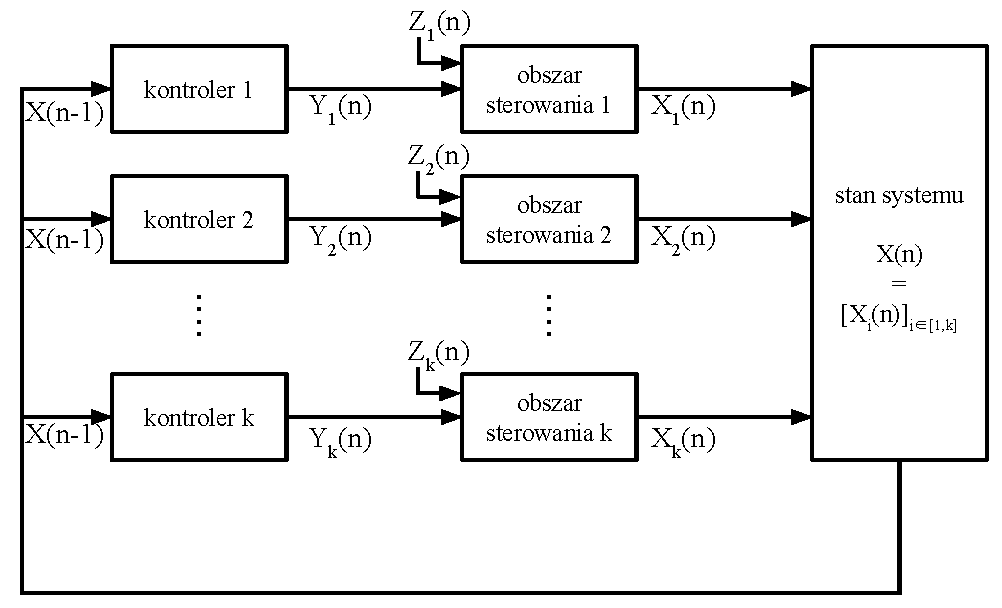
\includegraphics[width=0.8\textwidth]{images/model.pdf}
    \caption{Model systemu sterowania}
    \label{fig:model}
\end{figure}

\begin{equation}
	\begin{array}{c}
		U_i (n) = \left[ u_{i, j} (n) \right]_{j \in <1,s>}\\
		i \in <1,o>\\
		u_{i, j} (n) \in \left\{ \textrm{CZERWONY, CZERWONO-ZOLTY, ZIELONY, ZOLTY} \right\}\\
		o \in \mathbb{N}\\
		s \in \mathbb{N}
	\end{array}
\end{equation}

u_{i,j} (n) \textrm{ -- stan j-tego sygnalizatora w i-tym obszarze w chwili n}

o -- liczba obszarów sterowania

s -- liczba sygnalizatorów w obszarze

\begin{equation}
	\begin{array}{c}
		Z_i (n) = \left[ z_{i, j} (n) \right]_{j \in <1,r>}\\
		i \in <1,o>\\
		z_{i, j} (n) \in \mathbb{N}\\
		r \in \mathbb{N}
	\end{array}
\end{equation}

z_{i,j} (n) \textrm{ -- przepływ pojazdów z kierunku j w i-tym obszarze w chwili n}

r -- liczba wlotów do danego obszaru sterowania

\begin{equation}
	\begin{array}{c}
		X_i (n) = \left[
			\begin{array}{c}
				x_{i, j, 1} (n) \\ x_{i, j, 2} (n)
			\end{array}
		\right]_{j \in <1,s>}\\
		i \in <1,o>\\
		x_{i, j, 1} (n) \in \mathbb{N}\\
		x_{i, j, 2} (n) \in \mathbb{N}
	\end{array}
\end{equation}

x_{i, j, 1} (n) \textrm{ -- przepływ na dojeździe do j-tego sygnalizatora w i-tym obszarze}

x_{i, j, 2} (n) \textrm{ -- kolejka przed j-tym sygnalizatorem w i-tym obszarze}

\vspace{1.5cm}
Przepływy pojazdów mierzone są w pojazdach na godzinę, stany kolejek mierzone są w postaci liczby pojazdów.

\section{Wymagania sterowania ruchem drogowym}
\label{sec:model_ograniczenia}
Ograniczenia dotyczące sterowania ruchem drogowym zostały ustalone w rozporządzeniu ministra infrastruktury \cite{rozporzadzenie}. Wymagania te można sprowadzić do zestawu zasad dla programów sygnalizacji:
\subsection{Wymagania formalne}
\begin{itemize}
	\item Sygnały mogą być nadawane tylko w sekwencji czerwony, czerwono-żółty\footnote{sygnał czerwony z żółtym}, zielony, żółty, czerwony
	\item Długość sygnału żółtego powinna wynosić 3 sekundy
	\item Długość sygnału czerwono-żółtego powinna wynosić 1 sekundę
	\item Dla sygnalizacji akomodacyjnej/acyklicznej minimalna długość sygnału zielonego to 5 sekund
\end{itemize}

\subsection{Wymagania bezpieczeństwa}
Rozporządzenie definiuje podział par strumieni ruchu na strumienie niekolizyjne, strumienie kolizyjne o dopuszczalnym jednoczesnym zezwoleniu na ruch oraz strumienie kolizyjne o niedopuszczalnym jednoczesnym zezwoleniu na ruch.
Dla potrzeb opracowywanego systemu przyjęto, że strumienie kolizyjne nigdy nie mogą otrzymać jednoczesnego zezwolenia na ruch.

Zdefiniowano metodę obliczania czasów międzyzielonych dla kolizyjnych par strumieni. Zapewniają one minimalny czas w którym strumień ewakuujący się zdąży minąć punkt kolizji zanim osiągnie go strumień dojeżdżający. Minimalny czas międzyzielony wyznacza się na podstawie czasu trwania sygnału żółtego dla strumienia ewakuującego się, czasu ewakuacji strumienia ewakuującego się oraz czasu dojazdu strumienia dojeżdżającego.

\begin{equation}
	t^{min}_{m} (i,j) = t_{z} + t_{e} (i,j) - t_{d} (i,j)
\end{equation}

t^{min}_{m} (i,j) \textrm{ -- minimalny czas międzyzielony dla pary strumieni (i,j)}

t_{z} \textrm{ -- długość sygnału żółtego dla strumienia ewakuującego się}

t_{e} (i,j) \textrm{ -- czas ewakuacji strumienia i poza punkt kolizji ze strumieniem j}

t_{d} (i,j) \textrm{ -- czas dojazdu strumienia j do punktu kolizji ze strumieniem i}

t^{min}_{m} (i,j) = 0 \textrm{ jeśli obliczona wartość jest mniejsza od 0}

\begin{equation}
	t_{e} (i,j) = \frac{s_{e} (i,j) + I_p}{v_{e} (i)}
\end{equation}

s_{e} (i,j) \textrm{ -- droga strumienia ewakuującego się od linii zatrzymania do punktu kolizji}

I_p \textrm{ -- wartość wydłużająca drogę ewakuacji, dla strumienia pojazdów 10 metrów}

v_{e} (i) \textrm{ -- prędkość ewakuacji, prędkość dopuszczalna na wlocie, nie większa niż 14 m/s}

\begin{equation}
	t_{d} (i,j) = \frac{s_{d} (i,j)}{v_{d} (j)} + 1
\end{equation}

s_{d} (i,j) \textrm{ -- droga strumienia dojeżdżającego od linii zatrzymania do punktu kolizji}

v_{d} (i) \textrm{ -- prędkość ewakuacji, prędkość dopuszczalna na wlocie}